% http://dc-pubs.dbs.uni-leipzig.de/files/Rahm2000DataCleaningProblemsand.pdf
% https://www.quora.com/Can-I-automate-data-cleaning-using-machine-learning-algorithms

\chapter{Introduction\label{cha:chapter1}}

% https://books.google.de/books?id=2D0jBgAAQBAJ&pg=PA24&lpg=PA24&dq=%22die+ordnung+im+chaos+und+das+chaos+in+der+ordnung%22&source=bl&ots=rvYkaFGk-4&sig=IIxjTsPfpBmAEi8DBvmtHX0WE3Y&hl=en&sa=X&ved=0ahUKEwiM3ayxpvzUAhXKZFAKHc2mDV8Q6AEINjAD#v=onepage&q=%22die%20ordnung%20im%20chaos%20und%20das%20chaos%20in%20der%20ordnung%22&f=false

"Oder in the chaos and chaos in the order." This is how Osterhold describes one if the two essential directions of the chaos theory. Furthermore he claims, "processes, procedures or structures appearing very disordered only prove to be chaotic prior to they are analyzed further." This philosophical approach can be directly transfered to computer science, especially the field of information retrieval, data mining and data processing. 

\section{Motivation\label{sec:moti}}

% https://www.emc.com/leadership/digital-universe/2014iview/executive-summary.htm
% https://www.w3.org/TR/xmlschema-2/#boolean

The todays unbounded growth of information digitally available suggests a massive and chaotic collection of data. An in 2014 published report by EMC claims that the digitalized data grow by 100\% every two years and will reach 44 zettabytes (10\textsuperscript{21} bytes) by 2020 - as many stars as known in the universe. 
\\\\
Data in general, but also massive amounts of data, are only valuable if they are utilized appropriately. Gaining deeper insights is the point of transformation, visualization or calculation on data available. From a technical as well as an economical point of view a high degree of automation in data processing is required for maximizing the efficiency, especially when it comes to handling a high number of information entities. A large variety of software solutions are available and enable automated processing for numerous domains. The solutions capture all levels of abstraction and reach from end user desktop applications, e.g. Microsoft Excel, to low level software libraries, e.g. Pythons NumPy. Electronic data processing boils down to applied math and therefor relies on data of a deterministic structure. In computer science and mathematics there are well known specifications to transform and represent data in a computer understandable format. The canonical form, database normalization or schema definitions are some of them. They are primary beneficial for generalizing data representation on different abstraction levels, namely storing data in table-based format in files or specifying the order of bytes on hardware layer. A second evenly important aspect is the reduction of storage overhead when using predefined formats.
\\\\
Over the last years specifications being as old as the computers itself find less and less supporters and therefor their compliance. Mainly to mention here are the database and application level. Developments according to Moore's law and constantly decreasing  costs of volatile memory are the enabler of that ongoing trend. Computational power and high memory resources permit nowadays a by far more chaotic fashion of information storage. To perform analysis on data for reasonable time and resource costs in the past, it was essential to hold data in a well defined schema, i.e. the structure of the information entity with meta information about its attributes and types, and unique storage format on file level. Modern data management solutions and databases loosened that strict demands tremendously. Schema-less and document-orientated database management systems allow information entities with a deviating set of attributes to be stored. Data management and data retrieval systems even allow documents of different file and storage formats to be maintained. This trend develops in the favor of the users on application side. Overhead on schema definitions, restrictions due to backward compatibility or synchronization of parties and stakeholders almost vanish. The new development is very well received in technical development and opens new challenges in different research areas.
\\\\
The drawbacks of the a development have since been discovered by mostly consumers of such chaotic data. Not only the contemporary style of handling and storing information has its disadvantages but also data which already come in a well defined schema often do not fulfill the required granularity and purity of data for above mentioned use cases. In such applications a high amount of manual work for quality assurance has to be invested. Under the consideration of a rich landscape of different information entity formats data cleansing by hand, review of know-how owners or restructuration is done. This is only feasible on a low number of entities to be audited and becomes time and cost intense on big amounts of data. Initially claimed, that more powerful hardware resources even out the bumpy road is only true, if the the precision of the result must not meet a maximum. However, instances exist in which a best possible outcome on data analysis is indispensable. Exposure to end consumers, mathematical analysis or unification of a brought number of data sources are case that tend to demand the latter requirements to be met. 
\\\\
\textbf{User exposer of data:} A primary important aspect with regard to the need of clean data is the exposure to end users, for example in web shops or desktop applications. To make a service resilient against competitors it is fundamental to satisfy the most valuable resource, the end users. The paying customer who usually has a brought offer of services is most critical when it comes to functionality and appearance of the product. Insufficient information, unstructured layouts or poorly working features discourages a customer quickly. Those shortcomings can origin from problems in underlying data. E.g. product filters in a online shop do not apply correctly if the data representation in the target attributes is not groomed appropriately or characteristics are displayed in a inconsistent form. The data diversity in this case derives from, inter alia, different sources, e.g. different supplies or partners in an online shop.
\\\\
\textbf{Mathematical analysis:} For analysis of and calculation on messy data often a very high requirement of granularity and purity exists. In theoretical mathematics well defined sets of inputs and possible outputs for functions, the definition of algebraic structures and the scopes of algebraic axioms, or the consistency of vector spaces. This applies to for example techniques in the field of machine learning, especially to feature selection and feature engineering. Dimensions of feature vectors have to be assessed critically to avoid the 'course of dimensionality' and control their sparsity. Considering only subsets of data with sufficient quality will change results, e.g. on predictions based on a time series when certain time windows are removed due to the mentioned quality filters.
\\\\
\textbf{Unification of a brought number of data source:} There exist use cases and applications where it is indispensable to combine different data structures for the same entity from different sources. From a black-box point of view, a data aggregator only has one specific output but must combine a variety of source formats. Not only different information providers cause a data  inhomogeneity but also the gathering of the data plays a significant role. Facts like: information storages and data warehouses grow over time while compromises are made; technical and domain specifications for data management are not completely fulfilled; schemas vary, are underspecified or interpreted individually, impede a strict policy for homogeneous data. Information retrieval systems such as filter-engines, search-engines or recommendation systems face the stated problem and provide solutions to it. Some of the solutions imply a balance of manual configuration overhead on one side or reduced output quality on the other side. 
\\\\
XY claims that 80\% of effort in data analysis is devoted to data pre-processing and feature selection. That number indicates a large potential for maximizing the overall gain in the field of data processing. From the above addressed problems it can be seen that a large optimization leeway for automated data pre-processing exists. This space for optimization is considered as academic playground that motivates this work. Shifting the focus from data cleansing to actual data applications will be an enabler for quicker insight in data and lower the barrier for the development of data driven products.

\section{Objective and Problem statement\label{sec:objective}}
The outlined examples from the previous section sketched the problems currently present. In a more generalized aspect one can claim, that neither data from normalized sources, and even less data from schema-less sources often fulfill the required granularity and purity of data for above mentioned use cases. 

This thesis describes an approach to overcome the novel problems of diversity of available digital data. 


What kind of problem do you adress? Which issues do you try to solve? What solution do you propose? What is your goal?
'This thesis describes an approach to combining X and Y... The aim of this work is to...'

\section{Scope and Target\label{sec:scope}}
The target of this work is to analyze the current state of inhomogeneous data as outlined in the previous section, and assess this analysis. In a problem driven approach the findings are split into sub problems and key points with large optimization potential are identified. Those key points are discussed further and an overview of available techniques, technologies and approaches from different fields of computer science to tackle the state problems is provided.
\\\\
The main emphasis of this work is on the automation of pre-processing steps and ability to combine them in an adaptive manner. Therefor, a container framework is proposed. This framework must meet the latter requirements as well as simplifies the application of the works outcome. The key asset to be reduced with the proposed framework is manual overhead on data cleansing. Equally important is the extendability and adaptability of the tool set towards unseen data and temporal aspects. Concepts for a administration application in regards to quality assurance and framework maintainability is given. Those concepts are designed such that the remaining manual work can be reduced through minimizing the operators interactions. 
A second focus lies on the adaptability to an unstable environment. Predefined and agreed constrains and schemas do not last forever. A violation of that rule set does not necessarily mean that the data are corrupt and need to be cleaned and adapted. Under a different definition such data are in fact correct. This rises the need for a framework that adapts to the input data over time. Possible solutions can be taken from the field of machine learning as well as database management systems. Updating a learned models or collected data in an iterative approach is considered as promising. 
\\\\
On a less abstract level this work addresses the stated problems in the domain of food recipes. Here, the recipe is considered as information entity that comes in various semi-structured forms containing, among other attributes, a set of ingredients. The ingredients itself are combinations of a defined set of attributes that have a multitude of manifestations as well as non-deterministic order. References and similarities to other domains, e.g. product catalogs, are drawn and highlight to proof the ability to generalize of the proposed framework. A conclusion will assess the feasibility of such a system, review the performance result as well as address shortcomings.
\\\\
The overall target is to find a framework based solution that provides a tool set for automation of extraction essential key features of unequal information entities. As illustrated below the outcomes of this work can be adopted in applications that require high quality data. Figure \ref{fig:intro} shows the proposed framework as part of content based recommendation system utilized by 3rd party data.
\\
\begin{figure}[htb]
  \centering
  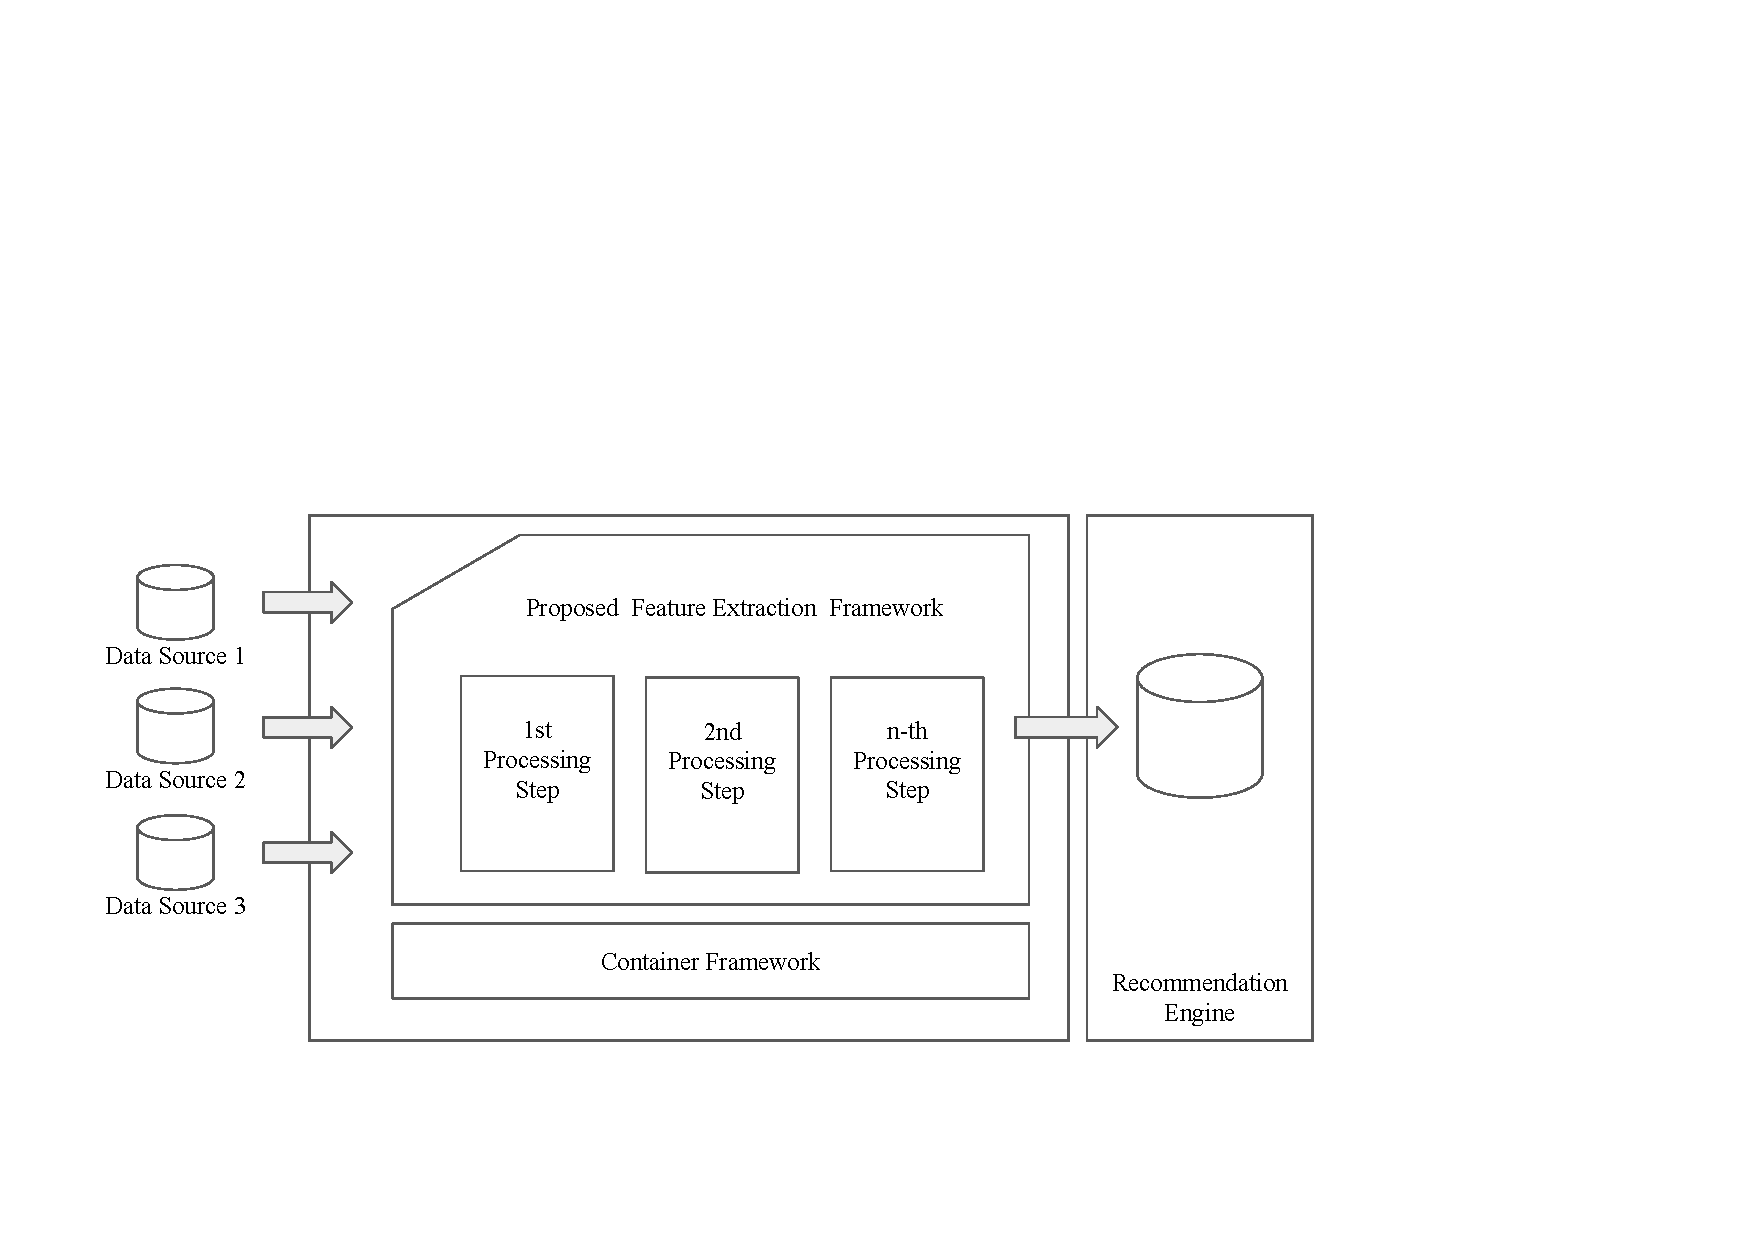
\includegraphics[width=0.9\textwidth]{framework-sketch.pdf}\\
  \caption{Feature extraction framework}\label{fig:intro}
\end{figure}

\section{Outline\label{sec:outline}}

The 'structure' or 'outline' section gives a brief introduction into the main chapters of your work. Write 2-5 lines about each chapter. Usually diploma thesis are separated into 6-8 main chapters. 
\\
\\
\noindent This example thesis is separated into 7 chapters.
\\
\\
\textbf{Chapter \ref{cha:chapter2}} is usually termed 'Related Work', 'State of the Art' or 'Fundamentals'. Here you will describe relevant technologies and standards related to your topic. What did other scientists propose regarding your topic? This chapter makes about 20-30 percent of the complete thesis.
\\
\\
\textbf{Chapter \ref{cha:chapter3}} analyzes the requirements for your component. This chapter will have 5-10 pages.
\\
\\
\textbf{Chapter \ref{cha:chapter4}} is usually termed 'Concept', 'Design' or 'Model'. Here you describe your approach, give a high-level description to the architectural structure and to the single components that your solution consists of. Use structured images and UML diagrams for explanation. This chapter will have a volume of 20-30 percent of your thesis.
\\
\\
\textbf{Chapter \ref{cha:chapter5}} describes the implementation part of your work. Don't explain every code detail but emphasize important aspects of your implementation. This chapter will have a volume of 15-20 percent of your thesis.
\\
\\
\textbf{Chapter \ref{cha:chapter6}} is usually termed 'Evaluation' or 'Validation'. How did you test it? In which environment? How does it scale? Measurements, tests, screenshots. This chapter will have a volume of 10-15 percent of your thesis.
\\
\\
\textbf{Chapter \ref{cha:chapter7}} summarizes the thesis, describes the problems that occurred and gives an outlook about future work. Should have about 4-6 pages.